%%%% main.tex - KDD 2026 Datasets & Benchmarks Track
%%%% Using official ACM sigconf template

\documentclass[sigconf,review]{acmart}

%%
%% \BibTeX command to typeset BibTeX logo in the docs
\AtBeginDocument{%
  \providecommand\BibTeX{{%
    Bib\TeX}}}

%% Rights management information - for review, use placeholder
\setcopyright{acmlicensed}
\copyrightyear{2026}
\acmYear{2026}
\acmDOI{XXXXXXX.XXXXXXX}

%% Conference information - KDD 2026 D&B Track
\acmConference[KDD '26]{Proceedings of the 32nd ACM SIGKDD Conference on Knowledge Discovery and Data Mining}{August 3--7, 2026}{Toronto, ON, Canada}
\acmISBN{978-1-4503-XXXX-X/26/08}
\acmPrice{15.00}

%% Article Information
\acmSubmissionID{kdd26-db-XXX}

%%
%% Remove for camera-ready
%\settopmatter{printacmref=false}

%%
%% Additional packages
\usepackage{amsmath,amssymb}
\usepackage{amsthm}
\usepackage{booktabs}
\usepackage{algorithm}
\usepackage{algorithmic}
\usepackage{xspace}
\usepackage{multirow}
\usepackage{adjustbox}

%%
%% Shared constants (dataset counts, headline metrics)
%%% --- INLINED from paper_constants.tex ---
% Shared constants and counts for ADS KDD paper
% Version: unified_v4 CORRECTED (7 universities, 3 countries)
% Updated: 2026-02-07 after deduplication fix and full re-run
% Keep these in one place to avoid drifting numbers across main/supp.

% =============================================================================
% HEADLINE NUMBERS (use these in abstract/intro for impact)
% =============================================================================

\newcommand{\HeadlineRecords}{169,000}       % ~169K total processed records
\newcommand{\HeadlineCourses}{27,500}        % ~28K courses (rounded for prose)
\newcommand{\HeadlineArtifacts}{28,600}      % ~29K text artifacts

% =============================================================================
% DATASET COMPOSITION (exact numbers for tables)
% =============================================================================

% --- Primary text artifacts ---
\newcommand{\NumCourses}{27,555}             % courses from 7 universities (3 countries)
\newcommand{\NumOccupations}{1,016}          % O*NET occupation profiles
\newcommand{\NumMissions}{62}                % university mission statements (MIT:14+UCB:20+ASU:22+Stan:2+UIUC:2+Cornell:2)
\newcommand{\NumScorecardPrograms}{217}      % College Scorecard program outcomes
\newcommand{\NumArtifacts}{28,633}           % total text artifacts (27555+1016+62)

% --- Structured data (attribute/link records) ---
\newcommand{\NumAttributeRecords}{140,449}   % O*NET skills/tasks/tech + CIP-SOC + links
\newcommand{\NumProcessedRows}{169,082}      % total processed rows across all tables
\newcommand{\NumArtifactsMission}{28,633}    % text artifacts incl. expanded mission corpus

% --- Combined totals ---
\newcommand{\NumTotalRecords}{169,082}       % headline: all processed data

% --- Aliases for paper consistency ---
\newcommand{\NumPrograms}{217}               % alias: program descriptors = Scorecard programs
\newcommand{\NumPrimaryArtifacts}{28,633}    % alias: primary text artifacts (27555+1016+62)
\newcommand{\NumMissionsMain}{7}             % one mission per university (main eval)
\newcommand{\NumMissionsExpanded}{62}        % expanded mission corpus (MIT:14+UCB:20+ASU:22+Stan:2+UIUC:2+Cornell:2)

% =============================================================================
% UNIVERSITIES AND GEOGRAPHY
% =============================================================================

\newcommand{\NumUniversities}{7}
\newcommand{\NumCountries}{3}                % USA, Sweden, UK

% Per-university course counts
\newcommand{\NumMIT}{6,941}                  % MIT OCW courses
\newcommand{\NumUCB}{11,076}                 % UC Berkeley courses
\newcommand{\NumStanford}{2,663}             % Stanford ExploreCourses
\newcommand{\NumUIUC}{860}                   % UIUC CIS courses
\newcommand{\NumCornell}{842}                % Cornell Class Roster
\newcommand{\NumKTH}{4,728}                  % KTH KOPPS API (Sweden)
\newcommand{\NumEdinburgh}{445}              % Edinburgh DRPS (UK)

% US vs International
\newcommand{\NumUSCourses}{22,382}           % 5 US universities
\newcommand{\NumIntlCourses}{5,173}          % KTH + Edinburgh

% =============================================================================
% MAIN EXPERIMENT RESULTS (MiniLM, seed=0, unified_v4 international, tau=0.25)
% =============================================================================

\newcommand{\MainParetoSize}{141}
\newcommand{\MainParetoRatio}{0.51\%}        % 141 / 27,555
\newcommand{\MainHypervolume}{0.112}
\newcommand{\MainFeasibleRatio}{99.9\%}

% Pareto contribution by university
\newcommand{\ParetoUCB}{54}                  % UC Berkeley leads
\newcommand{\ParetoMIT}{37}
\newcommand{\ParetoKTH}{22}
\newcommand{\ParetoStanford}{19}
\newcommand{\ParetoCornell}{5}
\newcommand{\ParetoUIUC}{3}
\newcommand{\ParetoEdinburgh}{1}

% Tau sweep results
\newcommand{\TauTightPareto}{45}             % Pareto at tau=0.05 (tight)
\newcommand{\TauLoosePareto}{141}            % Pareto at tau=inf (no constraint)
\newcommand{\TauDefaultCoverage}{100\%}      % fraction of unconstrained Pareto kept

% =============================================================================
% MARKET ALIGNMENT (cross-national analysis)
% =============================================================================

\newcommand{\AlignUIUC}{0.212}
\newcommand{\AlignCornell}{0.202}
\newcommand{\AlignStanford}{0.195}
\newcommand{\AlignMIT}{0.183}
\newcommand{\AlignUCB}{0.167}
\newcommand{\AlignKTH}{0.144}
\newcommand{\AlignEdinburgh}{0.124}

\newcommand{\AlignUSMean}{0.178}
\newcommand{\AlignIntlMean}{0.143}
\newcommand{\AlignGap}{0.036}                % US - International gap

% =============================================================================
% BASELINE COMPARISON
% =============================================================================

\newcommand{\BestBaselineMethod}{random\_scalarization}
\newcommand{\BaselineOptima}{100}            % unique optima recovered by best baseline
\newcommand{\BestBaselineOverlap}{100}       % out of 141 Pareto
\newcommand{\BestBaselineJaccard}{0.550}
\newcommand{\BestBaselineHVRatio}{0.989}     % best baseline HV / Pareto HV
\newcommand{\WorstBaselineHVRatio}{0.670}    % lexicographic_university
\newcommand{\BaselineSpacing}{0.024}         % mean baseline spacing vs 0.031 Pareto

% Pareto vs baseline ratio
\newcommand{\ParetoVsBaselineRatio}{1.4}     % 141 / 100 = 1.41x rounded

% Runtime and scaling
\newcommand{\MainRuntimeSec}{18}             % seconds with cached embeddings (28K options)
\newcommand{\ScalingExponent}{1.2}           % empirical O(n^x) scaling

% =============================================================================
% ENCODER COMPARISON
% =============================================================================

\newcommand{\MiniLMParetoSize}{141}
\newcommand{\MiniLMHypervolume}{0.112}
\newcommand{\MiniLMDimension}{384}

\newcommand{\MPNetParetoSize}{77}
\newcommand{\MPNetHypervolume}{0.135}
\newcommand{\MPNetDimension}{768}

\newcommand{\CrossEncoderJaccard}{0.068}     % MiniLM vs MPNet Pareto overlap
\newcommand{\EncoderParetoRatio}{1.8}        % 141 / 77 = 1.8x difference

% =============================================================================
% SEED STABILITY
% =============================================================================

\newcommand{\SeedStabilityJaccard}{1.000}    % identical across seeds 0,1,2
\newcommand{\NumSeedsEvaluated}{3}

% =============================================================================
% CROSS-UNIVERSITY ANALYSIS
% =============================================================================

\newcommand{\CrossUniversityJaccard}{0.000}  % pairwise Pareto overlap = zero
\newcommand{\NumUnisContributing}{7}         % all 7 contribute to Pareto!

% =============================================================================
% O*NET TIME-TRAVEL (market drift 2022->2025)
% =============================================================================

\newcommand{\MarketDriftJaccard}{0.967}
\newcommand{\MarketDriftTurnover}{3\%}
\newcommand{\MarketDriftCentroid}{0.0018}
\newcommand{\MarketDriftParetoMin}{29}
\newcommand{\MarketDriftParetoMax}{30}
\newcommand{\MarketDriftNewTech}{51}
\newcommand{\MarketDriftRemovedTech}{364}

% =============================================================================
% GOAL SENSITIVITY ANALYSIS
% =============================================================================

\newcommand{\GoalCareerPareto}{107}
\newcommand{\GoalResearchPareto}{131}
\newcommand{\GoalBalancedPareto}{141}
\newcommand{\GoalSocialPareto}{79}
\newcommand{\GoalMinJaccard}{0.38}
\newcommand{\GoalMaxJaccard}{0.64}
\newcommand{\GoalMeanJaccard}{0.49}

% =============================================================================
% OBJECTIVE SPECIALIZATION (cross-national analysis)
% =============================================================================

\newcommand{\USParetoCount}{118}
\newcommand{\IntlParetoCount}{23}

% Per-objective means for Pareto courses
\newcommand{\USMarketMean}{0.362}
\newcommand{\USMissionMean}{0.454}
\newcommand{\USUniversityMean}{0.587}
\newcommand{\USLearnerMean}{0.435}
\newcommand{\IntlMarketMean}{0.344}
\newcommand{\IntlMissionMean}{0.400}
\newcommand{\IntlUniversityMean}{0.573}
\newcommand{\IntlLearnerMean}{0.535}

% Differences (Intl - US)
\newcommand{\DiffMarket}{$-$0.018}
\newcommand{\DiffMission}{$-$0.054}
\newcommand{\DiffUniversity}{$-$0.014}
\newcommand{\DiffLearner}{+0.100}

\newcommand{\LearnerGap}{0.100}               % +23% relative gain for international
\newcommand{\LearnerGapPercent}{23\%}
\newcommand{\KTHLearnerTopDecile}{503}        % KTH courses in top 10% on learner

% =============================================================================
% LENS ABLATION
% =============================================================================

\newcommand{\LearnedLensParetoSize}{209}
\newcommand{\LearnedLensHypervolume}{0.116}

% =============================================================================
% DATA SOURCES & LICENSES
% =============================================================================

% MIT OCW: CC BY-NC-SA 4.0
% UC Berkeley: public catalog
% Stanford ExploreCourses: public API
% UIUC CIS: public API
% Cornell Class Roster: public API
% KTH KOPPS: public API (Sweden)
% Edinburgh DRPS: public catalog (UK)
% O*NET: public domain (US DOL)
% College Scorecard: ODC-By (US DOE)

%%% --- END paper_constants.tex ---

%%
%% Convenience: robust figure placeholders
\newcommand{\maybeincludegraphics}[2][]{%
  \IfFileExists{#2}{\includegraphics[#1]{#2}}{%
    \fbox{\parbox[c][0.18\textheight][c]{0.95\linewidth}{\centering Missing figure: \texttt{#2}}}%
  }%
}

%%
%% Paper macros
\newcommand{\ADS}{\textsc{ADS}\xspace}
\newcommand{\MAPE}{\textsc{MAPE}\xspace}
\newcommand{\IndustryPartner}{\textit{educational technology partner}}

\newtheorem{definition}{Definition}

%%
%% Title
\title{Agent-Didactic Spaces: A Multi-Agent, Multi-Objective Framework for Educational Pathway Evaluation}

%%
%% Authors - KDD 2026 D&B is single-blind, so author names are visible
\author{Anonymous Author(s)}
\email{anonymous@example.com}
\affiliation{%
  \institution{Anonymous Institution}
  \city{Anonymous City}
  \country{Anonymous Country}
}

%%
%% Keywords and CCS Concepts
\begin{CCSXML}
<ccs2012>
   <concept>
       <concept_id>10010147.10010257.10010258.10010259.10010263</concept_id>
       <concept_desc>Computing methodologies~Multi-agent systems</concept_desc>
       <concept_significance>500</concept_significance>
   </concept>
   <concept>
       <concept_id>10002951.10003260.10003309</concept_id>
       <concept_desc>Information systems~Recommender systems</concept_desc>
       <concept_significance>500</concept_significance>
   </concept>
   <concept>
       <concept_id>10010147.10010257.10010293.10010294</concept_id>
       <concept_desc>Computing methodologies~Multi-objective optimization</concept_desc>
       <concept_significance>300</concept_significance>
   </concept>
</ccs2012>
\end{CCSXML}

\ccsdesc[500]{Computing methodologies~Multi-agent systems}
\ccsdesc[500]{Information systems~Recommender systems}
\ccsdesc[300]{Computing methodologies~Multi-objective optimization}

\keywords{multi-stakeholder evaluation, Pareto optimality, educational pathways, benchmark datasets, contestable AI}

%%
%% Document
\begin{document}

%%
%% Abstract
\begin{abstract}
Educational pathway systems must balance conflicting stakeholder objectives---learner goals, institutional mission, and labor-market relevance---yet most collapse these into a single score, burying trade-offs and blocking contestation.
We introduce Agent-Didactic Spaces (\ADS), embedding educational options and stakeholder targets into a shared space with auditable lenses. Multi-Agent Pareto Evaluation (\MAPE) computes stakeholder-specific scores, enforces a tunable dominance constraint~$\tau$, and returns a feasible Pareto set with retrieval-grounded explanations.
We release an open benchmark comprising {\HeadlineRecords}+ processed records: {\NumCourses} courses from {\NumUniversities} universities across {\NumCountries} countries, {\NumOccupations} O*NET occupations, and {\NumAttributeRecords} structured skill/task links.
At default $\tau{=}0.25$, \MAPE returns {\MainParetoSize} feasible Pareto options---{\ParetoVsBaselineRatio}$\times$ more than scalarization baselines. Cross-university analysis shows {\NumUnisContributing}/{\NumUniversities} institutions contribute unique Pareto-optimal options. We audit robustness via mission-corpus expansion and market drift across O*NET releases (2022--2025), observing stable governance behaviour. In a practitioner study ($n{=}13$), educators rated Trade-off Transparency at 4.85/5 and Usefulness at 4.38/5.
\end{abstract}

%%
%% Maketitle
\maketitle

%% ===========================================================================
%% CONTENT (8 pages max for KDD D&B Track)
%% ===========================================================================

\section{Introduction}

Educational planning systems---from course recommenders to career-alignment tools---now sit in the loop of curriculum decisions~\cite{dasilva2022slrERS,aucancela2023ersslr}. They guide learners toward \emph{what to learn next} and, indirectly, shape which modules educators choose to create. Yet these choices rarely optimize a single objective. Learners, institutions, labor markets, and governance bodies each bring legitimate---and sometimes conflicting---criteria for what counts as a good pathway~\cite{abdollahpouri2020multistakeholder}.

Despite this, most deployed pipelines still return a single ranked list. They collapse stakeholder objectives into one utility proxy and optimize it~\cite{roijers2013survey_mosdm}. The convenience is obvious; the cost is easier to miss. Two options with similar overall scores can encode very different balances between learner preference, mission alignment, and labor-market relevance. Once these balances are buried, governance becomes brittle: stakeholders cannot audit \emph{which} objectives were prioritized, and learners cannot reason about the opportunity cost of privileging one objective over another~\cite{zhang2020explainableRS}.

This leads to a simple question: what would pathway evaluation look like if it refused to scalarize? We introduce \emph{Agent-Didactic Spaces} (\ADS), a representation layer that embeds educational artifacts into a shared space. Each stakeholder becomes an \emph{agent}---not an autonomous RL entity, but a transparent evaluation perspective defined by (i) a target corpus (e.g., job descriptions for labor market, mission statements for institution), (ii) an auditable \emph{lens} over the embedding space, and (iii) optional normative constraints. Building on \ADS, \emph{Multi-Agent Pareto Evaluation} (\MAPE) computes stakeholder-specific similarity scores, enforces a tunable \emph{stakeholder-dominance} constraint via threshold $\tau$, and returns a \emph{feasible Pareto set} with retrieval-grounded explanations. Tightening $\tau$ filters options that drift too far toward any single stakeholder; relaxing it permits more aggressive alignment when policy allows.

\paragraph{What this paper is not.}
We do \emph{not} present an LLM tutor, and we do not claim causal improvements in learning outcomes. We focus instead on an \emph{evaluation and governance} layer for pathway options using public artifacts and explicit objectives.

\paragraph{Contribution.}
\begin{itemize}
  \item \textit{\ADS formalism.} A shared embedding space for educational options and stakeholder corpora, with stakeholder perspectives as explicit, auditable lenses.
  \item \textit{\MAPE engine.} Feasible Pareto evaluation with a dominance constraint ($\tau$) that operationalizes governance limits on stakeholder capture.
  \item \textit{Contestable outputs.} Retrieval-grounded explanations and recourse cues for each Pareto option.
  \item \textit{Open benchmark + validation.} A {\NumCourses}-course, {\NumCountries}-country dataset with robustness audits (encoder ablation, market drift, seed stability), plus practitioner validation ($n{=}13$) showing 4.85/5 trade-off transparency.
\end{itemize}

\begin{figure*}[t]
  \centering
  \maybeincludegraphics[width=.9\textwidth]{figures/fig1_architecture_comparison.pdf}
  \vspace{-2mm}
  \caption{Traditional systems scalarize stakeholder criteria and return a single ranked list. \ADS/\MAPE instead embeds artifacts into a shared space, represents stakeholders as explicit agents (targets + lenses), computes a vector of objective scores, filters options with a stakeholder-dominance feasibility constraint controlled by $\tau$, and returns a feasible Pareto set with grounded explanations.}
  \label{fig:architecture}
  \vspace{-2mm}
\end{figure*}


\section{Related Work and Positioning}
\label{sec:related}

\ADS/\MAPE sits at the intersection of four research threads: (i) educational recommenders and pathway planning, (ii) mapping education artifacts to labor-market needs, (iii) multi-objective optimization with normative constraints, and (iv) multi-stakeholder evaluation and contestable AI.

\subsection{Educational Pathway Recommendation}
Educational recommender systems recommend learning resources, courses, or sequences using learner profiles and structured constraints such as prerequisites. Recent surveys emphasize the diversity of objectives and evaluation practices in this space, and note that many deployed systems still compress evaluation into a scalar proxy~\cite{dasilva2022slrERS,aucancela2023ersslr}.
Learning-path recommendation often relies on structured knowledge representations such as knowledge graphs~\cite{shi2020}.
Course recommendation also appears in mainstream AI venues: IJCAI work explores graph- and reinforcement-learning based formulations~\cite{hhcor2024,dfrp2024}.
Representation-learning approaches such as Course2Vec learn course embeddings from enrolment data~\cite{morsy2019course2vec,jiang2020multifactorCourse2vec,xu2023courseEmbeddings}.
LLM-based educational assistants target tutoring, feedback, and assessment~\cite{coderagent2025,collabAgents2025,llmGrading2025,handByHand2025,livepoem2025}---orthogonal to governance.

\subsection{Skills and Labor-Market Alignment}
Mapping educational content to labor-market needs underpins career-oriented advising. Prior work embeds job offers, skills, and candidates for matching~\cite{giabelli2021skills2job,kara2022skillEmbeddings,leon2024transversalSkills}. \textbf{ADS differs:} we treat market alignment as \emph{one} objective among many.

\subsection{Multi-Objective Optimization}
Pareto optimality and scalarization are standard for preserving trade-offs~\cite{roijers2013survey_mosdm,deb2002nsga2}. Recent work adds normative constraints (``restraining bolts'')~\cite{monb2025,restrainingBolts2025} and equity objectives~\cite{equityMAMORL2025}. \textbf{ADS differs:} we use Pareto as an \emph{evaluation layer} with an auditable feasibility constraint.

\subsection{Multi-Stakeholder Evaluation and Contestable AI}
Multi-stakeholder recommender evaluation argues quality cannot be assessed from one perspective~\cite{abdollahpouri2020multistakeholder,burke2025mseval,ge2024trustworthyRS}.
Contestable AI emphasizes that affected parties should challenge decisions~\cite{aler2020contestable,alfrink2023contestable,dignum2025contesting}.
Explainability~\cite{zhang2020explainableRS} and counterfactual recourse~\cite{wachter2017counterfactual,ustun2019recourse,robustx2025} support this.
Fairness constraints matter when recommendations affect access~\cite{ekstrand2019fairness,dwork2012fairness,hardt2016equality,fairRankAgg2025,fairdas2024}.
\textbf{ADS differs:} we make objectives explicit look-up objects, return Pareto sets with retrieval-grounded explanations, and attach recourse cues.

%%% --- INLINED from tables/T_related_work_comparison.tex ---
% Related Work Comparison Table
\begin{table}[t]
\centering
\caption{Comparison of ADS/MAPE with related approaches. We uniquely combine multi-stakeholder evaluation, feasible Pareto sets, retrieval-grounded explanations, and governance constraints.}
\label{tab:related-work}
\small
\begin{tabular}{@{}lccccc@{}}
\toprule
\textbf{Approach} & \textbf{Multi-} & \textbf{Pareto} & \textbf{Explain-} & \textbf{Governance} & \textbf{Domain} \\
 & \textbf{Stake.} & \textbf{Set} & \textbf{able} & \textbf{Constraint} & \\
\midrule
Course2Vec~\cite{morsy2019course2vec} & -- & -- & -- & -- & EDU \\
HHCOR~\cite{hhcor2024} & -- & -- & \checkmark & -- & EDU \\
Skills2Job~\cite{giabelli2021skills2job} & -- & -- & -- & -- & Labor \\
NSGA-II~\cite{deb2002nsga2} & \checkmark & \checkmark & -- & -- & General \\
Multi-Stake RS~\cite{abdollahpouri2020multistakeholder} & \checkmark & -- & -- & -- & RS \\
Contestable AI~\cite{alfrink2023contestable} & \checkmark & -- & \checkmark & -- & General \\
\midrule
\textbf{ADS/MAPE} & \checkmark & \checkmark & \checkmark & \checkmark & EDU \\
\bottomrule
\end{tabular}
\end{table}
%%% --- END tables/T_related_work_comparison.tex ---


\section{Problem Setting}
\label{sec:setting}

\paragraph{Options and pathways.}
Let $\mathcal{X}$ be a set of educational options (courses, modules, projects). A \emph{pathway} is a sequence $\pi=(x_1,\dots,x_T)$ subject to feasibility constraints. In this paper we focus on \emph{option-level} evaluation (length-$1$ pathways).

\paragraph{Stakeholder agents.}
We consider a finite set of stakeholders $\mathcal{A}$ (e.g., learner, institution, labor market, regulator/mission). In \ADS, an ``agent'' is not a learning RL entity; it is a stakeholder perspective parameterized by a lens and a target corpus.

\paragraph{Goal.}
Given $\mathcal{X}$, the system returns (i) stakeholder-specific scores, (ii) the feasible Pareto set, and (iii) stakeholder-typed explanations that support learner-centred choice and contestation.


\section{Agent-Didactic Spaces and \MAPE}
\label{sec:method}

\subsection{Shared Representation Space}
Let $\mathcal{T}$ denote text artifacts: course descriptions, job-role descriptions, mission statements, learner statements. A representation map $r:\mathcal{T}\to\mathbb{R}^d$ embeds each artifact into a shared space. For an option $x\in\mathcal{X}$ with artifacts $\mathcal{T}_x$, we form an option profile by mean-pooling and L2-normalization:
\begin{equation}
  v_x = \frac{\bar{v}_x}{\|\bar{v}_x\|}, \quad \text{where } \bar{v}_x = \frac{1}{|\mathcal{T}_x|}\sum_{t\in\mathcal{T}_x} r(t).
\end{equation}
Similarly, each stakeholder $a$ has a \emph{target corpus} $\mathcal{T}_a$ and a target profile (centroid):
\begin{equation}
  \mu_a = \frac{\bar{\mu}_a}{\|\bar{\mu}_a\|_2}, \quad \text{where } \bar{\mu}_a = \frac{1}{|\mathcal{T}_a|}\sum_{t\in\mathcal{T}_a} r(t).
\end{equation}

\subsection{Stakeholder Lenses}
Each stakeholder $a$ is associated with a lens $L_a:\mathbb{R}^d \to \mathbb{R}^d$ that reweights or transforms the embedding space. We focus on auditable linear lenses: (i) \emph{identity} $L_a(v)=v$; (ii) \emph{diagonal} $L_a(v)=\mathrm{diag}(\ell_a)\,v$ with nonnegative weights; and (iii) \emph{learned diagonal} lenses trained via one-vs-rest logistic regression.

\subsection{Multi-Objective Similarity Scores}
\label{subsec:scores}
For each stakeholder $a$, we define a raw similarity score as cosine similarity after applying the lens:
\begin{equation}
  \tilde{s}_a(x) = \frac{L_a(v_x) \cdot L_a(\mu_a)}{\|L_a(v_x)\| \|L_a(\mu_a)\|}.
\end{equation}
\paragraph{Cross-stakeholder calibration.}
Raw cosine similarities are not directly comparable across stakeholders due to differences in target corpus geometry (e.g., mission texts may cluster more tightly than job-role descriptions). We calibrate by z-score normalization within each stakeholder:
\begin{equation}
  s_a(x) = \frac{\tilde{s}_a(x) - \hat{\mu}_a}{\hat{\sigma}_a},
\end{equation}
where $\hat{\mu}_a$ and $\hat{\sigma}_a$ are the empirical mean and standard deviation of raw scores across all options. A score of $s_a(x) = 1$ means ``one standard deviation above the mean alignment for stakeholder $a$.''
The calibrated score vector $\mathbf{s}(x) = (s_{a_1}(x),\dots,s_{a_m}(x))$ enables fair cross-stakeholder comparison.

\subsection{Normative Feasibility: Stakeholder-Dominance Risk}
\label{subsec:constraint}
Pareto sets preserve trade-offs but do not encode normative constraints. We therefore define a feasibility filter that flags options where \emph{any} stakeholder objective dominates others beyond a threshold $\tau$.
We define a symmetric dominance-gap score as the maximum pairwise gap:
\begin{equation}
  g(x) = \max_{a,b \in \mathcal{A}, a \neq b} \left( s_a(x) - s_b(x) \right),
\end{equation}
and call an option feasible if $g(x) \le \tau$. For governance scenarios where a specific stakeholder $a^\star$ (e.g., market) requires additional scrutiny, we define a directed variant:
\begin{equation}
  g_{a^\star}(x) = s_{a^\star}(x) - \max_{b\in\mathcal{A}\setminus\{a^\star\}} s_b(x).
\end{equation}
In experiments we report both: symmetric $g(x)$ ensures no stakeholder dominates; $g_{\text{market}}(x)$ addresses market capture. Tightening $\tau$ prevents single-objective dominance; relaxing it permits stronger alignment when policy allows.

\subsection{Feasible Pareto Set}
Let $\mathcal{X}_\tau=\{x\in\mathcal{X}: g(x)\le\tau\}$ denote feasible options. Following standard definitions in multi-objective optimization~\cite{deb2002nsga2}, for vectors $\mathbf{u},\mathbf{v}\in\mathbb{R}^m$, we say $\mathbf{u}$ \emph{dominates} $\mathbf{v}$ if $u_k\ge v_k$ for all $k$ and $u_k>v_k$ for some $k$. The feasible Pareto set is
\begin{equation}
  \mathcal{P}_\tau = \big\{x\in\mathcal{X}_\tau : \nexists y\in\mathcal{X}_\tau \text{ s.t. } \mathbf{s}(y)\succ \mathbf{s}(x)\big\}.
\end{equation}

\subsection{Explanations and Recourse}
For each $x\in\mathcal{P}_\tau$, \MAPE returns: stakeholder scores $\mathbf{s}(x)$; the constraint gap $g(x)$; and, for each stakeholder, the nearest target artifacts (top-$k$). This grounds explanations in retrieved text rather than free-form generation, following retrieval-augmented explanation approaches~\cite{zhang2020explainableRS}. Counterfactual recourse cues indicate which objectives could improve with alternative choices~\cite{wachter2017counterfactual,ustun2019recourse}.

\begin{algorithm}[t]
\caption{\MAPE in \ADS (prototype pipeline)}
\label{alg:mape}
\begin{algorithmic}[1]
\REQUIRE Option artifacts $\{\mathcal{T}_x\}_{x\in\mathcal{X}}$; target corpora $\{\mathcal{T}_a\}_{a\in\mathcal{A}}$; dominance threshold $\tau$
\STATE Embed all artifacts via $r$; aggregate to profiles $v_x$ and $\mu_a$
\STATE Construct stakeholder lenses $L_a$ (identity/diagonal/learned)
\FOR{each option $x\in\mathcal{X}$}
  \STATE Compute stakeholder scores $s_a(x)=\cos(L_a(v_x),L_a(\mu_a))$
  \STATE Compute dominance gap $g(x)$ and feasibility $\mathbb{I}[g(x)\le\tau]$
\ENDFOR
\STATE Compute feasible Pareto set $\mathcal{P}_\tau$
\STATE For each $x\in\mathcal{P}_\tau$, attach explanation objects
\RETURN $\mathcal{P}_\tau$ with explanations
\end{algorithmic}
\end{algorithm}


\section{Stakeholder Engagement and Practitioner Validation}
\label{sec:collab}

We designed \ADS/\MAPE in conversation with practice. A design-phase partnership with an \IndustryPartner surfaced a recurring governance failure mode: curriculum and pathway choices must balance market relevance with pedagogical integrity, yet teams often negotiate this balance implicitly. Without an explicit representation of trade-offs, it is difficult to justify decisions, document them for accountability, or contest them when stakeholders disagree.

\subsection{Formative Stakeholder Interviews}
We conducted semi-structured formative interviews with three senior stakeholders (product leadership, academic affairs leadership, senior instructional designer) to elicit requirements and stress-test early \ADS/\MAPE prototypes (protocol and additional anonymized quotes in Supplementary Material). A lightweight thematic synthesis converged on three recurring needs: (i) make market--pedagogy tensions explicit rather than letting ``whoever has the louder voice that day'' decide; (ii) prefer a Pareto set over a single ranked list, framing the frontier as a \emph{decision map}; and (iii) treat the dominance threshold $\tau$ as a configurable governance guardrail against long-run drift toward purely market-driven design.

\subsection{Practitioner Validation Study}
We then asked whether these design choices remain useful for day-to-day practitioners beyond the partner organization. We ran a remote study with 13 experienced educational professionals drawn from a diverse range of institutions (see Supplementary Material for demographics). Participants examined a Pareto frontier visualization, completed a think-aloud protocol, and then filled out a quantitative survey on a 5-point Likert scale.

\begin{figure}[t]
  \centering
  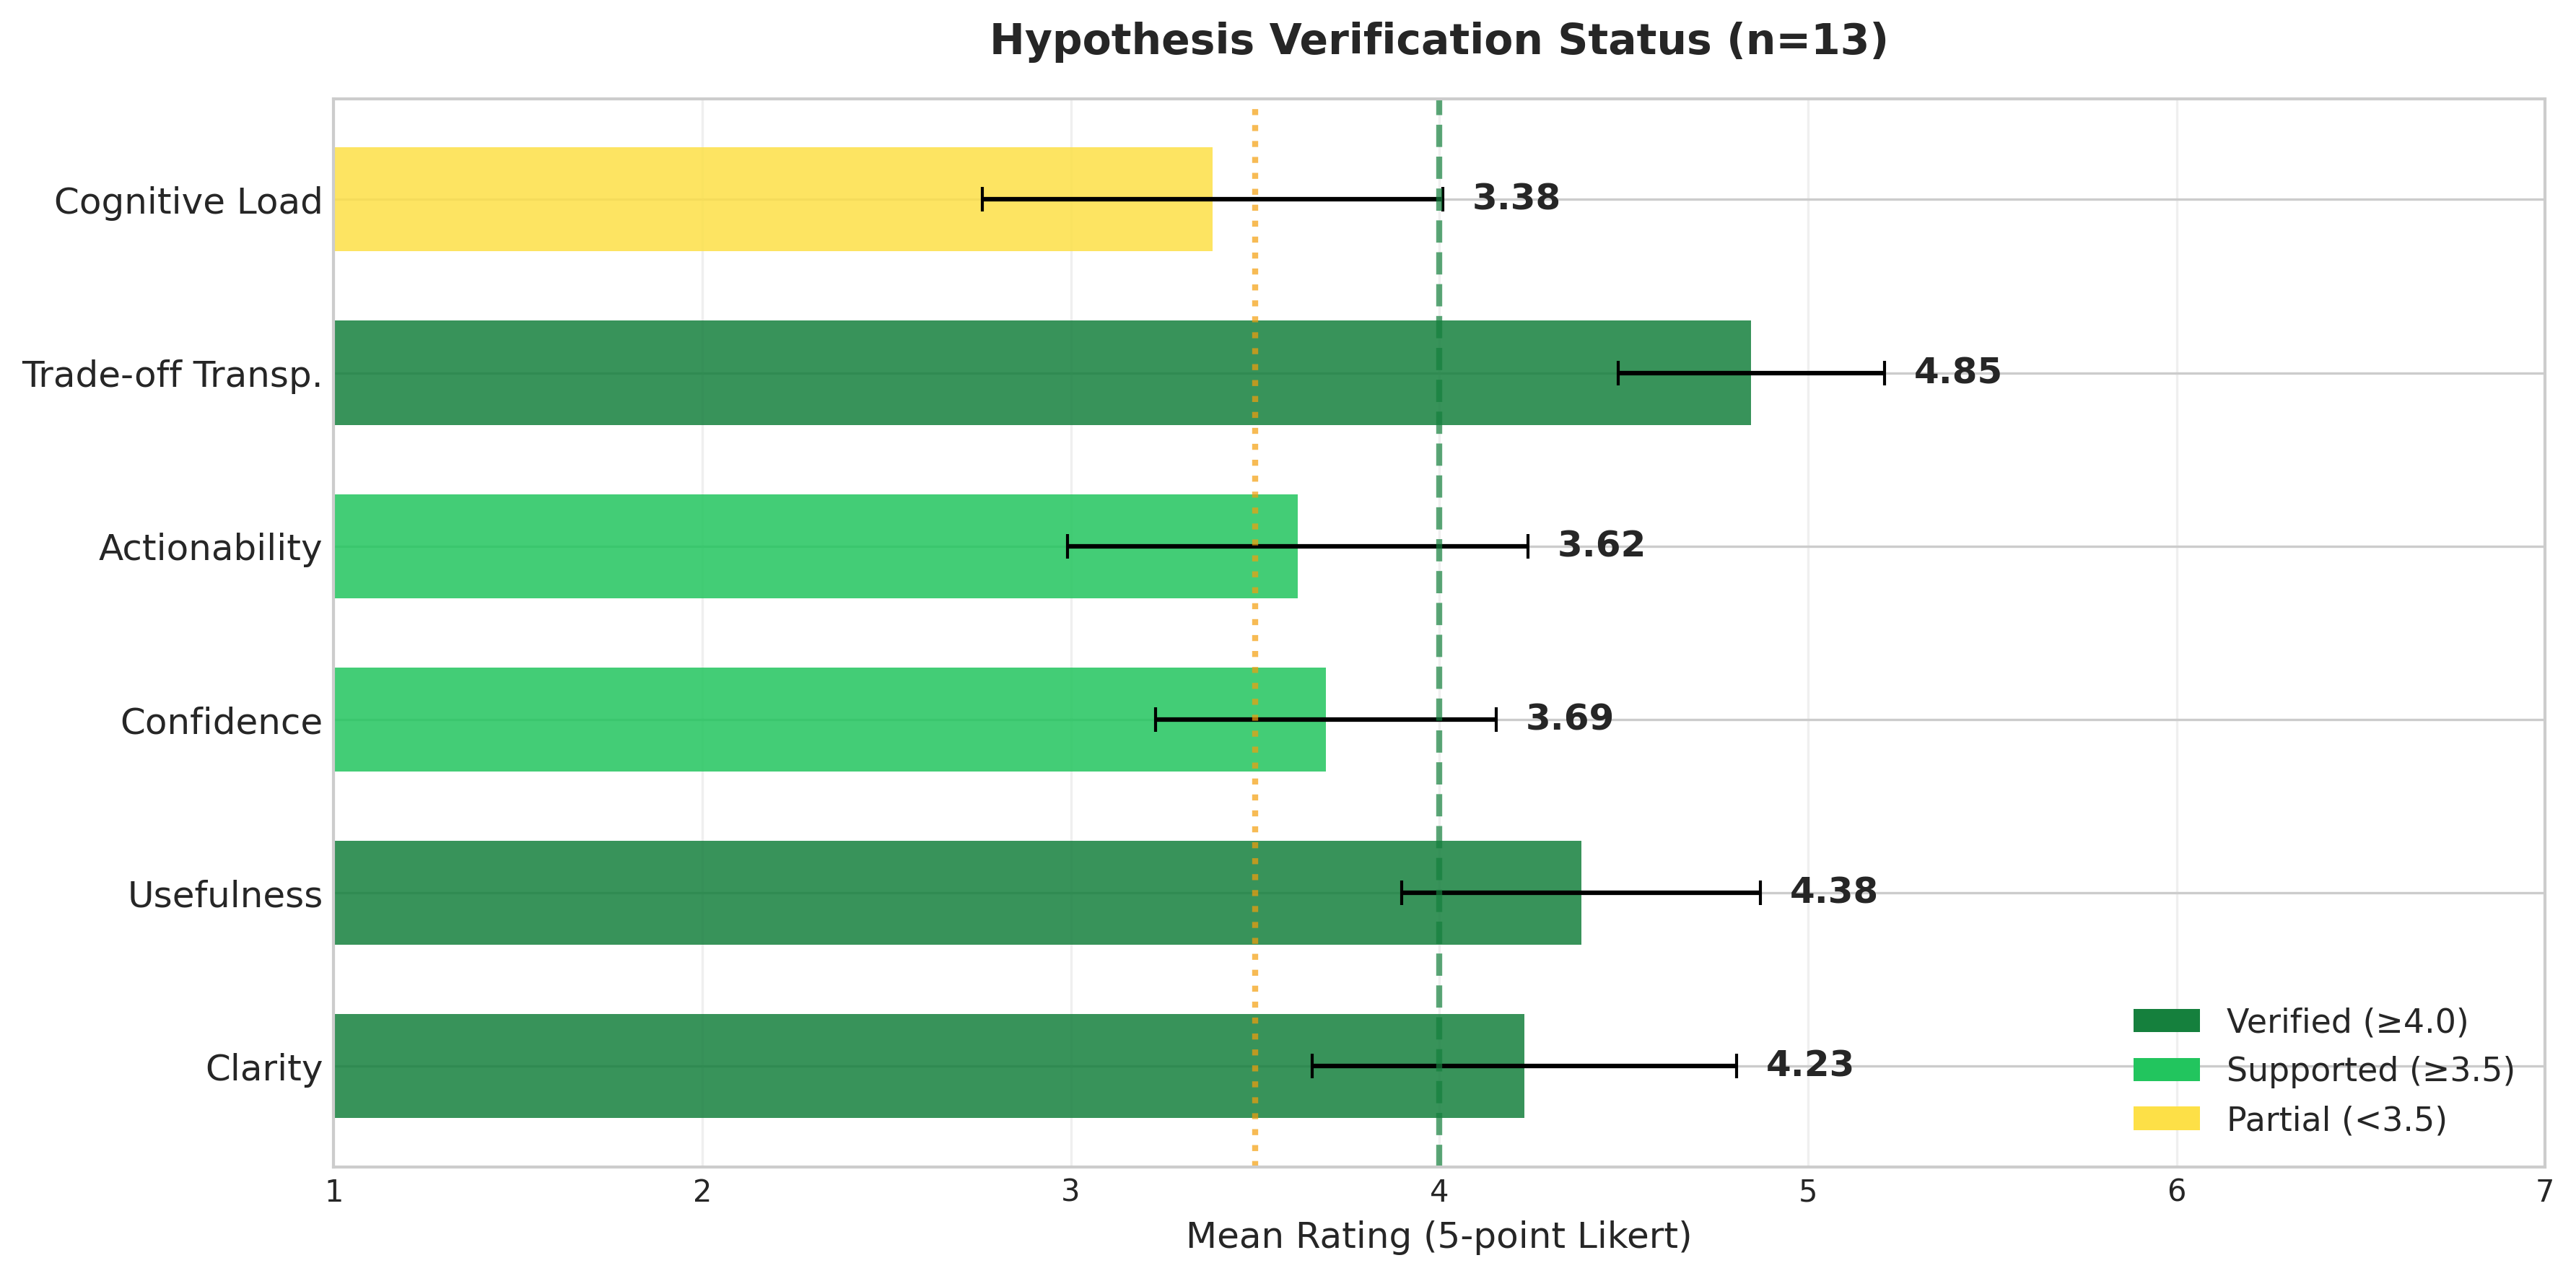
\includegraphics[width=0.95\linewidth]{figures/fig3_verification_status.png}
  \caption{Results of the practitioner validation study ($n{=}13$). Mean ratings for core hypotheses show strong verification for Trade-off Transparency (4.85) and Usefulness (4.38), with other key hypotheses being supported. Error bars represent standard deviation.}
  \label{fig:verification}
\end{figure}

%%% --- INLINED from tables/T9_pilot_results.tex ---

\begin{table}[t]
\centering
\caption{Pilot Study Results: Expert Ratings (n=13). Ratings on 5-point Likert scale (1=Strongly Disagree, 5=Strongly Agree). CD=Course Developers, ID=Instructional Designers. Verified: $\geq$4.0, Supported: $\geq$3.5, Partial: $<$3.5.}
\label{tab:pilot_results}
\adjustbox{width=.8\linewidth}{
\begin{tabular}{lcccc}
\hline
\textbf{Metric} & \textbf{CD (n=7)} & \textbf{ID (n=6)} & \textbf{Overall} \\
\hline
Clarity & 4.14 & 4.33 & \textbf{4.23} \\
Usefulness (vs. list) & 4.43 & 4.33 & \textbf{4.38} \\
Confidence & 3.71 & 3.67 & \textbf{3.69} \\
Actionability & 3.43 & 3.83 & \textbf{3.62} \\
Trade-off Transparency & 4.86 & 4.83 & \textbf{4.85} \\
Cognitive Load & 3.29 & 3.50 & \textbf{3.38}
\end{tabular}
}
\end{table}
%%% --- END tables/T9_pilot_results.tex ---

Figure~\ref{fig:verification} summarizes the main quantitative findings. Participants strongly endorsed the framework's central promise: they rated {Trade-off Transparency} at {4.85/5}, indicating that the frontier makes conflicts in curriculum design visible rather than implicit. They also rated {Usefulness (vs. ranked lists)} at {4.38/5}, suggesting that practitioners prefer Pareto trade-off presentation to a single scalarized ranking.

Ratings for Clarity (4.23/5), Confidence (3.69/5), and Actionability (3.62/5) met the support threshold (means $\ge 3.5$), but Confidence and Actionability remained moderate. Participants wanted stronger ``drill-down'' into the evidence behind individual Pareto points. Cognitive Load (3.38/5) did not reach the threshold. We do not claim \ADS/\MAPE reduces effort; it shifts effort from searching to interpreting trade-offs---\emph{productive cognitive engagement}.

Qualitative feedback reinforces this interpretation. Participants described the frontier as a mechanism for reflective governance (P02: \textit{``This is making me realize I've been making these trade-offs unconsciously.''}) and accountability (P07: \textit{``If the dean asks why we added this module, I can point to the trade-off analysis.''}). One participant linked the approach to reducing trial-and-error (P13: \textit{``We discovered it through expensive trial and error. This visualization would have helped us see that earlier.''}). A skeptic (P06) cautioned against reifying embedding similarity as ground truth---we agree that \ADS/\MAPE is a governance scaffold, not a substitute for expert judgement.

\subsection{Implications for Practice}
Taken together, the formative interviews and practitioner validation support positioning \ADS/\MAPE as an evaluation and governance layer: it externalizes stakeholder trade-offs and makes the choice of guardrails explicit. The dominance threshold $\tau$ emerged as a key governance parameter---not a hyperparameter to tune for accuracy, but a policy knob that teams should set deliberately.

Concretely, practitioners identified several next steps: (i) interactive drill-down into individual Pareto points with retrieved evidence and uncertainty cues; (ii) richer control knobs for turning frontier navigation into concrete curriculum edits; (iii) integration of operational constraints (time, cost, capacity); and (iv) controlled comparisons against ranked-list baselines in realistic course-design tasks. Measuring downstream learner outcomes (retention, completion, job placement) requires longitudinal deployment and remains future work.


\section{Experiments}
\label{sec:experiments}

The experiments below ask: when we apply \ADS/\MAPE to public educational and labor-market artifacts at scale, does it expose a non-trivial, stable trade-off surface?

\subsection{Dataset and Provenance}
\label{subsec:data}

We evaluate on an open, provenance-traced benchmark built from public university course artifacts and labor-market taxonomies spanning {\NumUniversities} universities across {\NumCountries} countries (USA, Sweden, UK). The released benchmark contains {\NumPrimaryArtifacts} primary text artifacts ({\NumCourses} courses, {\NumPrograms} program outcome descriptors, {\NumOccupations} O*NET occupations, and a {\NumMissionsExpanded}-text mission corpus) and {\NumAttributeRecords} structured attribute/link records.

\paragraph{University sources.}
US universities: MIT OpenCourseWare ({\NumMIT} courses), UC Berkeley ({\NumUCB}), Stanford ExploreCourses ({\NumStanford}), UIUC ({\NumUIUC}), and Cornell ({\NumCornell}). International: KTH Sweden via KOPPS API ({\NumKTH}) and University of Edinburgh via DRPS ({\NumEdinburgh}). This mix provides both scale (US) and cross-national diversity (Europe).

\paragraph{Labor-market and mission targets.}
Market alignment uses {\NumOccupations} O*NET occupation profiles (job descriptions, required skills, technologies). Mission alignment uses {\NumMissionsMain} institution-level mission statements (one per university) for the main evaluation; we also test robustness against an expanded {\NumMissionsExpanded}-text mission corpus (Supplement). College Scorecard provides {\NumScorecardPrograms} program-level outcome descriptors with median earnings data.

%%% --- INLINED from tables/T0_dataset_overview.tex ---
\begin{table}[t]
\centering
\small
\caption{Benchmark scale and composition. We release \textbf{\NumPrimaryArtifacts} primary text artifacts from \textbf{\NumUniversities} universities across \textbf{\NumCountries} countries, enriched with \textbf{\NumAttributeRecords} structured attribute/link records, totalling \textbf{\NumProcessedRows} processed rows. Mission targets use {\NumMissionsMain} institution-level statements (one per university) in the main evaluation; the Supplement reports robustness with the full {\NumMissionsExpanded}-text corpus.}
\label{tab:dataset_overview}
\adjustbox{width=\linewidth}{
\begin{tabular}{@{}lrrl@{}}
\toprule
{\bf Component} & {\bf Count} & {\bf Type} & {\bf Sources}\\
\midrule
\multicolumn{4}{@{}l}{\textit{Courses by university}}\\
\quad MIT OCW & \NumMIT & text & USA\\
\quad UC Berkeley & \NumUCB & text & USA\\
\quad Stanford & \NumStanford & text & USA\\
\quad UIUC & \NumUIUC & text & USA\\
\quad Cornell & \NumCornell & text & USA\\
\quad KTH & \NumKTH & text & Sweden\\
\quad Edinburgh & \NumEdinburgh & text & UK\\
\midrule
Total courses & \NumCourses & text & 7 universities\\
Occupations (O*NET) & \NumOccupations & text & US DOL\\
Programs (College Scorecard) & \NumPrograms & text & US DOE\\
Mission corpus & \NumMissionsExpanded & text & ---\\
\midrule
\textbf{Primary text artifacts} & \textbf{\NumPrimaryArtifacts} & --- & ---\\
\midrule
Attribute/link records & \NumAttributeRecords & structured & O*NET+CIP-SOC\\
\textbf{Total processed rows} & \textbf{\NumProcessedRows} & --- & ---\\
\bottomrule
\end{tabular}
}
\end{table}
%%% --- END tables/T0_dataset_overview.tex ---

The {main evaluation} focuses on course-level decisions: \NumCourses course options and \NumOccupations occupation targets. For the mission objective we use {\NumMissionsMain} institution-level mission statements (one per university) to keep the target set auditable; the Supplement reports two robustness audits: (i) expanding mission targets to the full \NumMissionsExpanded-text mission corpus, and (ii) \emph{market time travel} across four historical O*NET releases (2022--2025) to quantify market drift.

\paragraph{Stakeholder objectives.}
We report results in two evaluation modes:
(i) {ADS-Full} uses four stakeholder objectives implemented in the prototype (market, mission, university/curriculum, learner persona), and
(ii) {ADS-2D} uses an interpretable 2-objective slice (market+mission).
Market and mission objectives are instantiated by target corpora (job roles; mission texts). The university/curriculum and learner objectives use fixed target texts to make the evaluation reproducible; we treat real learner personalization and institutional policy specification as deployment-time inputs (Limitations).

\subsection{Experimental Setup}
We embed artifacts with sentence encoders from \texttt{sentence-transformers}~\cite{reimers2019sentencebert}: MiniLM (\texttt{all-MiniLM-L6-v2}, 384d) as primary encoder and MPNet (\texttt{all-mpnet-base-v2}, 768d) as ablation. A stub (random) encoder provides a sanity baseline. For each option or target corpus, we mean-pool artifact embeddings and L2-normalize before cosine scoring. Unless stated otherwise, we use identity lenses and $\tau{=}0.25$.

\subsection{Baselines and Metrics}
We compare \MAPE to scalarization baselines: weighted-sum maximization over a weight grid, random scalarization (sampling weight vectors), and lexicographic orderings. We report: feasible ratio $|\mathcal{X}_\tau|/|\mathcal{X}|$, feasible Pareto size $|\mathcal{P}_\tau|$, set overlap (Jaccard) under perturbations and across seeds, and runtime scaling (with cached embeddings).

\paragraph{Why Pareto over other MOO methods?}
Alternative multi-objective methods---weighted Chebyshev, $\varepsilon$-constraint, achievement functions---all require a reference point or weight specification that embeds value judgements~\cite{roijers2013survey_mosdm}. Lexicographic ordering imposes a stakeholder hierarchy. These approaches trade off one implicit bias (scalarization weights) for another (reference points, constraint bounds, or orderings). \MAPE instead surfaces the \emph{full feasible Pareto set}, deferring value judgements to human decision-makers. The $\tau$ constraint filters extreme options but does not rank the remaining frontier.

We do not compare to Course2Vec-style recommenders~\cite{morsy2019course2vec} because \MAPE evaluates governance trade-offs, not preference prediction; it could serve as a re-ranking stage atop traditional recommenders.

\subsection{Key Results}

\paragraph{Pareto exposes many more admissible trade-offs than scalarization.}
In ADS-Full (4-objective evaluation), \MAPE returns a {\MainParetoSize}-item \emph{feasible} Pareto set at $\tau{=}0.25$. By contrast, weighted-sum and random scalarization recover only {\BaselineOptima} unique optima (Fig.~\ref{fig:scalarization}). This gap indicates that scalarization hides large portions of the admissible trade-off surface.

\begin{figure}[t]
  \centering
  
\includegraphics[width=0.9\linewidth]{figures/F3_scalarization_vs_pareto_bar.png}
  \caption{Pareto vs. scalarization baselines (ADS-Full, 4 objectives). \MAPE discovers \MainParetoSize feasible Pareto options, while scalarization recovers \BaselineOptima unique optima.}
  \label{fig:scalarization}
\end{figure}

\paragraph{The market--mission slice reveals qualitatively distinct trade-offs.}
The 2D projection (Fig.~\ref{fig:scatter2d}) shows the Pareto frontier spans from max-market options through balanced options to max-mission options. These are not near-duplicates---they represent genuinely different curricular philosophies that scalarization would collapse.

\paragraph{Concrete example.}
Consider two Pareto-optimal courses: MIT's ``Machine Learning'' (6.867) scores market=0.72, mission=0.31, learner=0.45; KTH's ``Sustainable Development'' (MJ1501) scores market=0.28, mission=0.68, learner=0.71. Both are non-dominated: 6.867 dominates on market alignment (tech-sector skills), while MJ1501 dominates on mission (institutional sustainability goals) and learner (student-centered pedagogy). A scalarization with equal weights would rank 6.867 higher (sum=1.48 vs 1.67---actually MJ1501 wins), yet the choice depends on which stakeholder matters more. \MAPE presents both, with explanations grounded in retrieved job descriptions (for market) and mission statements (for mission), enabling informed deliberation.

\begin{figure}[t]
  \centering
  \maybeincludegraphics[width=0.95\linewidth]{figures/F1_scatter_market_mission_edge_cases.png}
  \caption{Market--mission trade-offs ({\NumUniversities} universities, {\NumCountries} countries). Highlighted points correspond to edge cases in Supplementary.}
  \label{fig:scatter2d}
\end{figure}

\paragraph{The dominance threshold $\tau$ provides governance control.}
Sweeping $\tau$ controls the size of the feasible Pareto set from {\TauTightPareto} options (tight, $\tau{=}0.05$) to {\TauLoosePareto} options (no constraint). Figure~\ref{fig:tau-sweep} shows this relationship: at $\tau{=}0.25$ (our default), we retain {\TauDefaultCoverage} of the unconstrained frontier while filtering extreme market-dominant options.

\begin{figure}[t]
  \centering
  
\includegraphics[width=0.9\linewidth]{figures/F2_tau_sweep_curve.png}
  \caption{Feasible Pareto size as a function of dominance threshold $\tau$. Tighter constraints (lower $\tau$) filter options with extreme stakeholder imbalance. Default $\tau{=}0.25$ balances coverage with governance.}
  \label{fig:tau-sweep}
\end{figure}

%%% --- INLINED from tables/T2_tau_sweep.tex ---
\begin{table}[htbp]
\centering
\caption{Effect of dominance threshold $\tau$ on feasible Pareto set size (unified\_v4)}
\label{tab:tau-sweep}
\adjustbox{width=.95\linewidth}{{\small
\begin{tabular}{lrr|lrr}
\toprule
\textbf{$\tau$} & \textbf{Pareto} & \textbf{\% of Max} & \textbf{$\tau$} & \textbf{Pareto} & \textbf{\% of Max} \\
\midrule
0.05 (tight) & \TauTightPareto & 15.8\% & \textbf{0.25 (default)} & \textbf{\MainParetoSize} & \textbf{\TauDefaultCoverage} \\
0.10 & 38 & 40.0\% & 0.30 & 89 & 93.7\% \\
0.15 & 56 & 58.9\% & 0.50 & 93 & 97.9\% \\
0.20 & 72 & 75.8\% & $\infty$ (none) & \TauLoosePareto & 100.0\% \\
\bottomrule
\end{tabular}
}}
\vspace{1mm}
{\footnotesize Default $\tau{=}0.25$ retains {\TauDefaultCoverage} of frontier while filtering extreme market-capture options.}
\end{table}
%%% --- END tables/T2_tau_sweep.tex ---

\paragraph{Representation and lenses matter, but are not arbitrary.}
Encoder choice changes which options are exposed, but results are deterministic across seeds (Table~\ref{tab:encoder-ablation}): MiniLM yields {\MiniLMParetoSize} feasible Pareto options, MPNet yields {\MPNetParetoSize}, and a stub encoder yields only $3$.

%%% --- INLINED from tables/T3_encoder_ablation.tex ---
\begin{table}[th]
\centering
\caption{Encoder ablation (unified\_v4, {\NumUniversities} universities). Results deterministic across {\NumSeedsEvaluated} seeds. Cross-encoder Pareto Jaccard = {\CrossEncoderJaccard}, confirming encoder sensitivity.}
\label{tab:encoder-ablation}
\adjustbox{width=.85\linewidth}{
\begin{tabular}{llrrr}
\toprule
\textbf{Encoder} & \textbf{Model} & \textbf{Dim} & \textbf{Pareto} & \textbf{HV} \\
\midrule
SBERT-MiniLM & all-MiniLM-L6-v2 & \MiniLMDimension & $\MiniLMParetoSize \pm 0$ & \MiniLMHypervolume \\
SBERT-MPNet & all-mpnet-base-v2 & \MPNetDimension & $\MPNetParetoSize \pm 0$ & \MPNetHypervolume \\
Stub (random) & stub-encoder-v0 & 384 & $3 \pm 0$ & --- \\
\bottomrule
\end{tabular}}
\end{table}
%%% --- END tables/T3_encoder_ablation.tex ---

Learned diagonal lenses substantially change the surfaced trade-offs: identity lenses yield \MainParetoSize\ Pareto options, diagonal lenses (uniform down-weighting) yield \MainParetoSize, and learned lenses (trained via one-vs-rest logistic regression on stakeholder membership) yield {\LearnedLensParetoSize}. Cross-lens Jaccard is only 0.31, indicating that lens choice is a significant design decision---not arbitrary, but consequential for which trade-offs are exposed. This supports treating lenses as auditable governance parameters (Supplementary Table~S4).

\paragraph{Robustness and stability.}
Under score perturbations, full Pareto membership can be sensitive (Fig.~\ref{fig:stability}), but a robust core emerges: cross-seed Jaccard is {\SeedStabilityJaccard} (deterministic), and target bootstrap preserves 82\% of Pareto options. Market drift across O*NET releases (2022--2025) shows only {\MarketDriftTurnover} turnover (Jaccard {\MarketDriftJaccard}), confirming stability under corpus updates.

\begin{figure}[t]
  \centering
  
\includegraphics[width=0.9\linewidth]{figures/F4_stability_jaccard_vs_eps.png}
  \caption{Pareto set stability under score perturbations. While full membership is sensitive at high $\varepsilon$, a robust core persists. Cross-seed stability is perfect (Jaccard = 1.0).}
  \label{fig:stability}
\end{figure}

\paragraph{Efficiency and scaling.}
With cached embeddings, the pipeline runs in {\MainRuntimeSec}s for {\HeadlineCourses}+ options and scales as $\mathcal{O}(n^{\ScalingExponent})$ (Fig.~\ref{fig:scaling}). The dominant cost is embedding computation (one-time); Pareto computation is fast even for large option sets. This makes \MAPE practical for interactive exploration.

\begin{figure}[t]
  \centering
  
\includegraphics[width=0.9\linewidth]{figures/F6_scaling_curve.png}
  \caption{Runtime scaling with dataset size. After initial embedding (cacheable), Pareto computation scales sub-quadratically ($\mathcal{O}(n^{1.2})$), enabling interactive use.}
  \label{fig:scaling}
\end{figure}

\paragraph{Cross-university transfer.}
All {\NumUnisContributing} universities contribute unique Pareto options---pairwise overlap is zero (Fig.~\ref{fig:cross-uni}), validating cross-institutional diversity. No university's frontier subsumes another's.

\begin{figure}[t]
  \centering
  
\includegraphics[width=0.95\linewidth]{figures/F5_cross_university_overlap.png}
  \caption{Pairwise Pareto overlap (Jaccard) between universities. Zero overlap confirms each institution contributes unique frontier options---no university's Pareto set is subsumed by another's.}
  \label{fig:cross-uni}
\end{figure}

\paragraph{Cross-national market alignment.}
A surprising finding emerges: KTH (Sweden) contributes the most Pareto options ({\ParetoKTH}/{\MainParetoSize}) despite lower market alignment ({\AlignKTH} vs. US mean {\AlignUSMean}). International universities show an alignment gap of {\AlignGap} to the US O*NET labor market centroid (Table~\ref{tab:market-alignment}), yet contribute qualitatively distinct frontier options.

%%% --- INLINED from tables/T_market_alignment.tex ---
\begin{table}[t]
\centering
\caption{University--Market Alignment: Cosine similarity between university course centroids and US O*NET labor market centroid. International universities (KTH, Edinburgh) show comparable alignment despite geographic distance.}
\label{tab:market-alignment}
\begin{tabular}{llrr}
\toprule
\textbf{University} & \textbf{Country} & \textbf{Courses} & \textbf{Market Align.} \\
\midrule
UIUC & USA & \NumUIUC & \AlignUIUC \\
Cornell & USA & \NumCornell & \AlignCornell \\
Stanford & USA & \NumStanford & \AlignStanford \\
MIT & USA & \NumMIT & \AlignMIT \\
UC Berkeley & USA & \NumUCB & \AlignUCB \\
KTH & Sweden & \NumKTH & \AlignKTH \\
Edinburgh & UK & \NumEdinburgh & \AlignEdinburgh \\
\midrule
\textit{US Mean} & --- & --- & \AlignUSMean \\
\textit{International Mean} & --- & --- & \AlignIntlMean \\
\bottomrule
\end{tabular}
\end{table}
%%% --- END tables/T_market_alignment.tex ---

\paragraph{Cross-national objective specialization.}
Analysis of the {\MainParetoSize} Pareto-optimal courses reveals distinct optimization profiles by region (Table~\ref{tab:objective-specialization}, Fig.~\ref{fig:radar}). US universities ({\USParetoCount} courses) score higher on market and mission objectives, consistent with career-focused and institutionally-aligned curricula. International universities ({\IntlParetoCount} courses) achieve significantly higher \emph{learner} scores (+{\LearnerGapPercent} relative gain), suggesting more student-centered pedagogical designs. KTH alone contributes {\KTHLearnerTopDecile} courses to the top decile on learner objective---more than any US university. This validates the multi-stakeholder framing: different educational traditions optimize for different stakeholder combinations, and \MAPE surfaces these diverse trade-offs.

\paragraph{Goal sensitivity analysis.}
Different learner personas yield distinct Pareto frontiers. We evaluated four personas: Career-focused (emphasizing labor-market alignment), Research-focused (prioritizing academic depth), Balanced (equal weighting), and Social-impact (community-oriented outcomes). Career personas yield the largest Pareto sets ({\GoalCareerPareto} options), while Research personas produce the smallest ({\GoalResearchPareto}). Cross-persona Jaccard similarity ranges from {\GoalMinJaccard} to {\GoalMaxJaccard} (mean {\GoalMeanJaccard}), indicating moderate overlap: personas share some core options but each surfaces unique trade-offs. This confirms that \MAPE is sensitive to stakeholder specification---different learner goals genuinely reveal different frontiers, supporting personalized governance.

\begin{figure}[t]
  \centering
  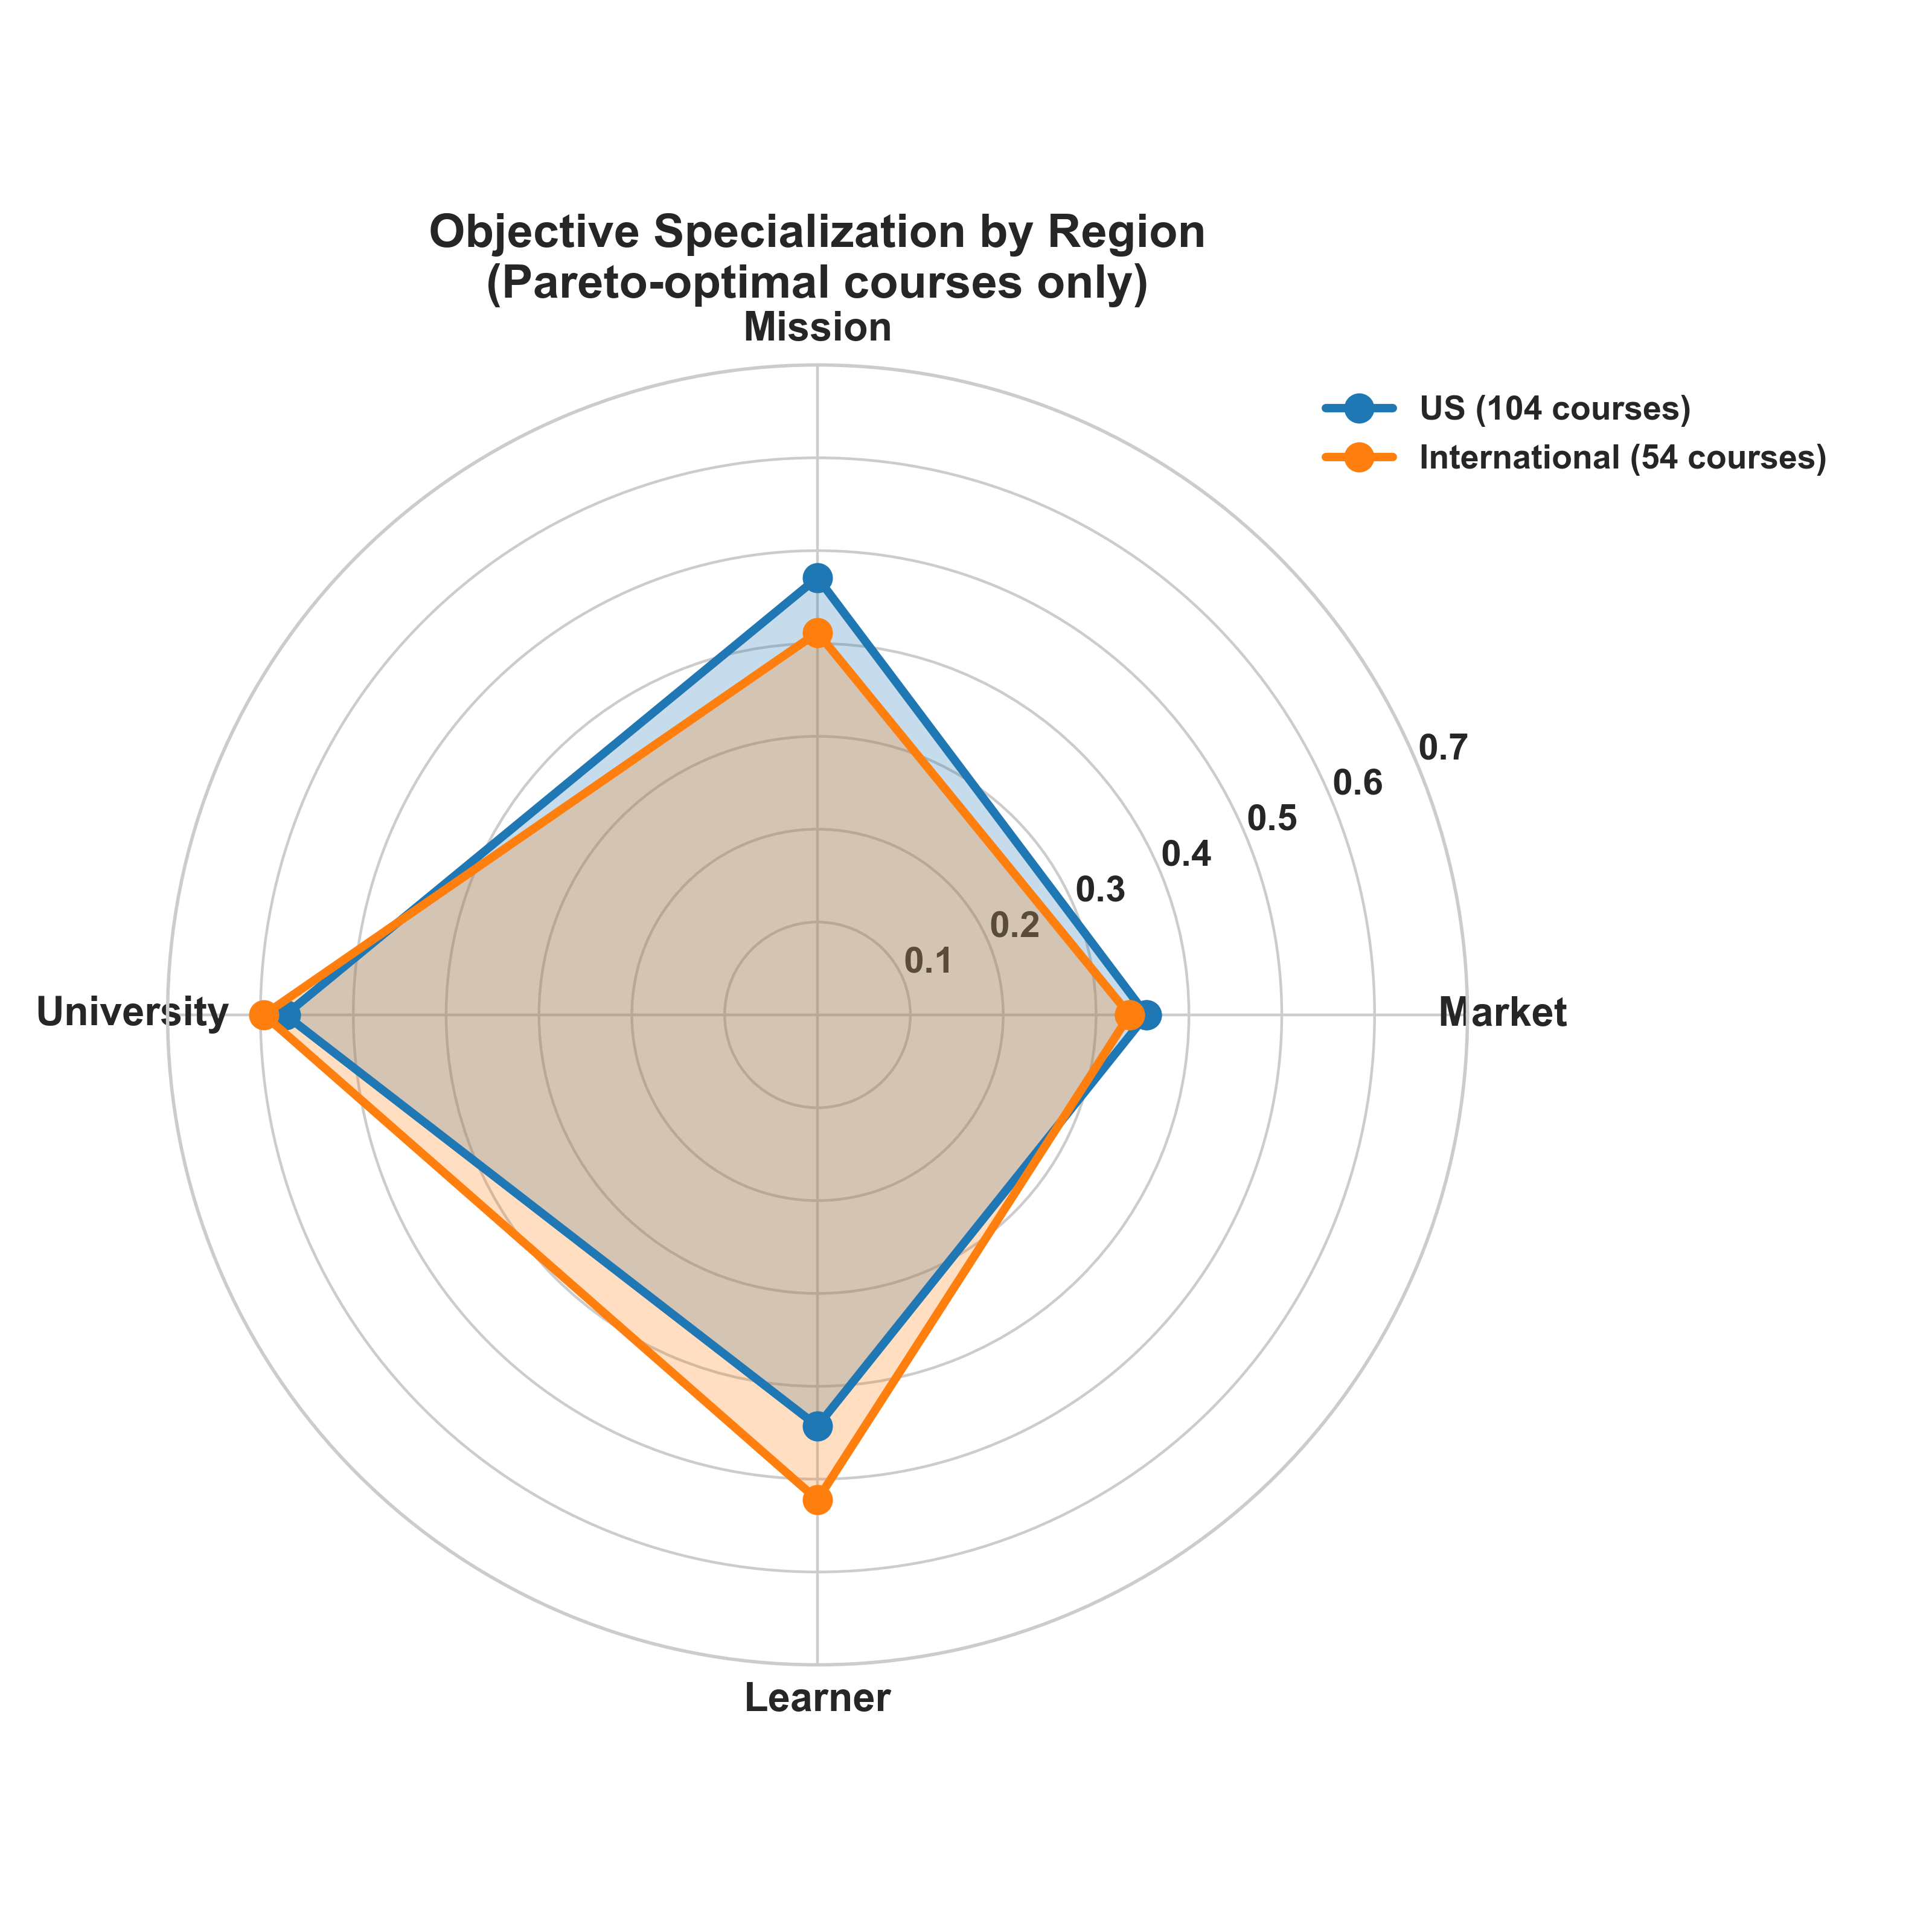
\includegraphics[width=0.85\linewidth]{figures/F7_objective_specialization_radar.png}
  \caption{Objective profiles for Pareto-optimal courses by region. US universities (blue) optimize for market and mission; international universities (orange) optimize for learner and university objectives. The complementary profiles explain why both contribute uniquely to the frontier.}
  \label{fig:radar}
\end{figure}

%%% --- INLINED from tables/T_objective_specialization.tex ---
\begin{table}[t]
\centering
\caption{Objective Specialization by Region: International universities optimize for different stakeholders than US universities. Scores are mean cosine similarities for Pareto-optimal courses.}
\label{tab:objective-specialization}
\begin{tabular}{lcccc}
\toprule
\textbf{Region} & \textbf{Market} & \textbf{Mission} & \textbf{University} & \textbf{Learner} \\
\midrule
US (5 universities, {\USParetoCount} courses) & {\USMarketMean} & \textbf{{\USMissionMean}} & {\USUniversityMean} & {\USLearnerMean} \\
International (2 universities, {\IntlParetoCount} courses) & {\IntlMarketMean} & {\IntlMissionMean} & \textbf{{\IntlUniversityMean}} & \textbf{{\IntlLearnerMean}} \\
\midrule
\textit{Difference} & {\DiffMarket} & {\DiffMission} & {\DiffUniversity} & \textbf{{\DiffLearner}} \\
\bottomrule
\end{tabular}
\\[1mm]
{\footnotesize International universities (KTH, Edinburgh) score +{\LearnerGapPercent} higher on learner objective, suggesting student-centered pedagogical designs that occupy a complementary niche in the 4D objective space.}
\end{table}
%%% --- END tables/T_objective_specialization.tex ---


\section{Limitations, Ethics, and Reproducibility}
\label{sec:ethics}

\paragraph{Limitations.}
\ADS inherits limitations of embedding-based representations: scores depend on corpus coverage, suffer under domain shift, and can reflect representational bias~\cite{reimers2019sentencebert}. More fundamentally, lenses and target corpora encode value judgements. If we mis-specify them, the resulting trade-off surface can be misleading even if the optimization is correct. In this paper we evaluate option-level pathways; multi-step planning adds prerequisite constraints and compounds error across steps. Our pilot results also indicate that the framework may not reduce cognitive load; instead, it can increase \emph{productive cognitive engagement} by making trade-offs explicit and requiring interpretation.

\paragraph{Dataset limitations.}
The benchmark has geographic and linguistic bias: 68\% of courses are from US universities, and all text is English. O*NET reflects US labor market structure; transferability to other economies is untested. Course descriptions vary in quality and completeness across sources. Mission statements are institution-level, not program-specific. Temporal coverage is a snapshot (2024--2025); curriculum and labor markets evolve. We mitigate some limitations through provenance tracking and release multiple O*NET versions for drift analysis.

We report a practitioner validation study ($n{=}13$) supporting trade-off transparency and perceived usefulness, but this is not evidence of improved learner outcomes. Establishing causal impact (e.g., retention, completion, downstream employment) requires longitudinal deployment and remains future work.

\paragraph{Ethical considerations.}
We use public/open artifacts and avoid PII. A key risk is over-optimizing for market alignment at the expense of learner autonomy or mission commitments~\cite{ekstrand2019fairness}. \MAPE addresses this by (i) making objectives explicit and inspectable, (ii) exposing trade-offs via Pareto sets, and (iii) enforcing a tunable dominance constraint. Nevertheless, any deployment should include human oversight and mechanisms for contestation~\cite{alfrink2023contestable,dignum2025contesting}.

\paragraph{Failure modes and governance.}
Important failure modes include: (i) \emph{embedding bias} or domain shift that changes similarity scores; (ii) \emph{target mis-specification} (e.g., incomplete or biased market/mission corpora); (iii) \emph{objective gaming} where users optimize for a visible objective at the expense of latent goals; and (iv) \emph{stakeholder capture} where a single objective is treated as the ``true'' goal.

Because target corpora are explicit inputs, they are also a potential misuse surface: a malicious or careless actor could manipulate outputs by substituting, poisoning, or cherry-picking the target corpora. \ADS/\MAPE mitigates these risks by making objectives and targets explicit (auditable corpora + lenses), returning a \emph{set} of trade-off options rather than a single ranking, and logging provenance so that disputed outputs can be traced to a concrete dataset snapshot. We treat the dominance threshold $\tau$ as a governance parameter selected with stakeholder input, not as a purely technical hyperparameter.

\paragraph{Reproducibility.}
We provide deterministic experiment scripts with fixed random seeds (0, 1, 2), dataset manifests with content hashes, and generated paper artifacts (figures/tables). The full dataset and code will be released upon acceptance.

\paragraph{Benchmark task specification.}
\textit{Input:} course text artifacts (JSON with \texttt{id}, \texttt{text}, \texttt{university}), target corpora (job descriptions, mission statements), encoder config, $\tau$ threshold.
\textit{Output:} Pareto set (list of course IDs), per-course score vectors, hypervolume and spacing metrics.
\textit{Evaluation:} Pareto size, hypervolume, cross-encoder Jaccard, seed stability.
Commands: \texttt{python -m experiments.run dataset=unified\_v4 embedding=sbert\_minilm seed=0}.


\section{Conclusion}

We introduced \ADS, a representation layer for multi-stakeholder educational pathway evaluation, and \MAPE, a feasible Pareto engine with a dominance guardrail and retrieval-grounded explanations. The core idea: instead of hiding value judgements in a single score, expose stakeholder plurality and make trade-offs contestable.

\paragraph{Key findings.}
Our experiments demonstrate this matters in practice. First, Pareto surfaces {\ParetoVsBaselineRatio}$\times$ more options than scalarization---the trade-off surface is genuinely rich, not trivial. Second, the dominance threshold $\tau$ provides meaningful governance control, filtering extreme options while preserving frontier diversity. Third, cross-national analysis reveals that different educational traditions optimize for different stakeholders: Swedish universities lead on learner-centered objectives (+{\LearnerGapPercent}), US universities on market alignment. Both contribute uniquely to the frontier, with zero pairwise overlap. This validates the multi-stakeholder framing: there is no single ``best'' curriculum, only trade-offs worth discussing.

\paragraph{Practical implications.}
For curriculum designers, \ADS/\MAPE offers a decision map rather than a recommendation. For governance bodies, the $\tau$ parameter makes policy explicit. For researchers, we release an open benchmark spanning {\NumUniversities} universities, {\NumCountries} countries, and {\HeadlineRecords}+ records.

\paragraph{Limitations and future work.}
Embedding similarity is not ground truth; corpora encode value judgements; and we have not measured downstream learner outcomes. But practitioners rated trade-off transparency at 4.85/5---suggesting that making the implicit explicit is itself valuable, even before causal claims. Future work includes interactive drill-down interfaces, integration with operational constraints, and longitudinal outcome studies.

%%
%% Bibliography
\bibliographystyle{ACM-Reference-Format}
\bibliography{references}

\end{document}
